%%
%% Copyright 2022 OXFORD UNIVERSITY PRESS
%%
%% This file is part of the 'oup-authoring-template Bundle'.
%% ---------------------------------------------
%%
%% It may be distributed under the conditions of the LaTeX Project Public
%% License, either version 1.2 of this license or (at your option) any
%% later version.  The latest version of this license is in
%%    http://www.latex-project.org/lppl.txt
%% and version 1.2 or later is part of all distributions of LaTeX
%% version 1999/12/01 or later.
%%
%% The list of all files belonging to the 'oup-authoring-template Bundle' is
%% given in the file `manifest.txt'.
%%
%% Template article for OXFORD UNIVERSITY PRESS's document class `oup-authoring-template'
%% with bibliographic references
%%

\documentclass[namedate,numsec,webpdf,modern,large]{oup-authoring-template}

%\onecolumn % for one column layouts

%\usepackage{showframe}

\graphicspath{{Fig/}}

% line numbers
%\usepackage[mathlines, switch]{lineno}
%\usepackage[right]{lineno}

\theoremstyle{thmstyleone}%
\newtheorem{theorem}{Theorem}%  meant for continuous numbers
%%\newtheorem{theorem}{Theorem}[section]% meant for sectionwise numbers
%% optional argument [theorem] produces theorem numbering sequence instead of independent numbers for Proposition
\newtheorem{proposition}[theorem]{Proposition}%
%%\newtheorem{proposition}{Proposition}% to get separate numbers for theorem and proposition etc.
\theoremstyle{thmstyletwo}%
\newtheorem{example}{Example}%
\newtheorem{remark}{Remark}%
\theoremstyle{thmstylethree}%
\newtheorem{definition}{Definition}

\usepackage{acronym}
\acrodef{CRN}[CRN]{chemical reaction network}
\acrodef{DSL}[DSL]{domain-specific language}
\acrodef{GPU}[GPU]{graphical processing unit}
\acrodef{GUI}[GUI]{graphical user interface}
\acrodef{IDE}[IDE]{integrated development environment}
\acrodef{JIT}[JIT]{just-in-time}
\acrodef{ODE}[ODE]{ordinary differential equation}
\acrodef{PyPI}[PyPI]{Python package index}
\acrodef{RHS}[RHS]{right-hand side}
\acrodef{SBML}[SBML]{Systems Biology Markup Language}
\acrodef{SDE}[SDE]{stochastic differential equation}
\acrodef{DDE}[DDE]{delay differential equation}
\acrodef{TPU}[TPU]{tensor processing unit}

\usepackage{tcolorbox}
\newenvironment{CodeInput}{\begin{tcolorbox}[title=input,boxrule=0pt]}{\end{tcolorbox}}
\newenvironment{CodeOutput}{\begin{tcolorbox}[title=output,boxrule=0pt]}{\end{tcolorbox}}

\usepackage{fancyvrb}
\DefineVerbatimEnvironment{Highlighting}{Verbatim}{commandchars=\\\{\}}
\newcommand{\KeywordTok}[1]{\textcolor[rgb]{0.00,0.13,1.00}{#1}}
\newcommand{\ClassTok}[1]{\textcolor[rgb]{0.27,0.56,0.65}{#1}}
\newcommand{\OperatorTok}[1]{\textcolor[rgb]{0.00,0.00,0.00}{#1}}
\newcommand{\VariableTok}[1]{\textcolor[rgb]{0.00,0.06,0.50}{#1}}
\newcommand{\ValueTok}[1]{\textcolor[rgb]{0.13,0.57,0.41}{#1}}
\newcommand{\FunctionTok}[1]{\textcolor[rgb]{0.47,0.37,0.15}{#1}}
\newcommand{\IDETok}[1]{\textcolor[rgb]{0.58,0.58,0.58}{#1}}
\newcommand{\NormalTok}[1]{\textcolor[rgb]{0.00,0.06,0.50}{#1}}
\newcommand{\CommentTok}[1]{\textcolor[rgb]{0.00,0.50,0.00}{#1}}
\newcommand{\StringTok}[1]{\textcolor[rgb]{0.70,0.27,0.27}{#1}}

\begin{document}

\journaltitle{Journal Title Here}
\DOI{DOI HERE}
\copyrightyear{2022}
\pubyear{2019}
\access{Advance Access Publication Date: Day Month Year}
\appnotes{Paper}

\firstpage{1}

%\subtitle{Subject Section}

\title[Poincaré and SimBio: a versatile and extensible Python ecosystem for modeling systems]{Poincaré and SimBio: a versatile and extensible Python ecosystem for modeling systems}

\author[1,2]{Mauro Silberberg\ORCID{0000-0000-0000-0000}}
\author[3]{Henning Hermjakob\ORCID{0000-0000-0000-0000}}
\author[3]{Rahuman S. Malik-Sheriff\ORCID{0000-0000-0000-0000}}
\author[1,2,$\ast$]{Hernán E. Grecco\ORCID{0000-0000-0000-0000}}

\authormark{Author Name et al.}

\address[1]{\orgname{Universidad de Buenos Aires, Facultad de Ciencias Exactas y Naturales, Departamento de Física}, \orgaddress{\state{Buenos Aires}, \country{Argentina}}}
\address[2]{\orgname{CONICET - Universidad de Buenos Aires, Instituto de Física de Buenos Aires (IFIBA)}, \orgaddress{\state{Buenos Aires}, \country{Argentina}}}
\address[3]{\orgdiv{European Bioinformatics Institute}, \orgname{European Molecular Biology Laboratory (EMBL-EBI)}, \orgaddress{\street{Wellcome Genome Campus}, \state{Cambridge}, \country{UK}}}

\corresp[$\ast$]{Corresponding author. \href{email:hgrecco@df.uba.ar}{hgrecco@df.uba.ar}}

\received{Date}{0}{Year}
\revised{Date}{0}{Year}
\accepted{Date}{0}{Year}

%\editor{Associate Editor: Name}

%\abstract{
%\textbf{Motivation:} .\\
%\textbf{Results:} .\\
%\textbf{Availability:} .\\
%\textbf{Contact:} \href{name@email.com}{name@email.com}\\
%\textbf{Supplementary information:} Supplementary data are available at \textit{Journal Name}
%online.}

\abstract{
  \Acfp{CRN} play a pivotal role in diverse fields
  such as systems biology, biochemistry, chemical engineering, and epidemiology.
  High-level definitions of \acp{CRN} enables to use various simulation approaches,
  including deterministic and stochastic methods,
  from the same model.
  However,
  existing Python tools for simulation of \ac{CRN} typically wrap external C/C++ libraries for
  model definition, translation into equations and/or numerically solving them,
  limiting their extensibility and integration with the broader Python ecosystem.
  In response, we developed Poincaré and SimBio,
  two novel Python packages for simulation of dynamical systems and \acp{CRN}.
  Poincaré serves as a foundation for dynamical systems modelling,
  while SimBio extends this functionality to \acp{CRN},
  including support for the \ac{SBML}.
  Poincaré and SimBio are developed as pure Python packages
  enabling users to easily extend their simulation capabilities
  by writing new or leveraging other Python packages.
  Moreover, this does not compromise the performance,
  as code can be \ac{JIT} compiled with Numba.
  Our benchmark tests using curated models from the BioModels repository
  demonstrate that these tools may provide a potentially
  superior performance advantage compared to other existing tools.
  Additionally, to ensure a user-friendly experience,
  our packages use standard typed modern Python syntax that provides a seamless integration with \acp{IDE}.
  Our Python-centric approach significantly enhances code analysis, error detection, and refactoring capabilities,
  positioning Poincaré and SimBio as valuable tools for the modelling community.
}
\keywords{poincare, SimBio, Python, ODE}
\acresetall % reset acronyms after abstract

% \boxedtext{
% \begin{itemize}
% \item Key boxed text here.
% \item Key boxed text here.
% \item Key boxed text here.
% \end{itemize}}

\maketitle


\section{Introduction}

\Acp{CRN} are a fundamental concept of modelling in numerous fields
including systems biology, biochemistry, chemical engineering and epidemiology.
They are comprised of a set of chemical species or biological entities
and a set of reactions that mediate transformations between them.
These systems can be simulated through multiple approaches:
deterministic \acp{ODE} to model macroscopic behavior,
\acp{SDE} to model microscopic fluctuations,
and jump processes (Gillespie-like simulations) to account for the discreteness of populations.
Instead of directly writing the equations for each of these formulations,
which is error-prone and difficult to reuse,
these models can be \emph{defined} in a higher-level description
that can be \emph{translated} into equations for the different types of simulations
and, then, \emph{solved} numerically.

Several tools already exist to \emph{define}, \emph{translate} and \emph{solve} \acp{CRN}.
BioSimulators.org \cite{shaikhBioSimulatorsCentralRegistry2022},
a registry of simulation tools,
lists at least 15 softwares categorized under Python including
COPASI \cite{hoopsCOPASICOmplexPAthway2006},
Tellurium \cite{choiTelluriumExtensiblePythonbased2018} and
PySB \cite{lopezProgrammingBiologicalModels2013}.
COPASI is a standalone software with a \ac{GUI}
that is widely used for its user-friendly interface and comprehensive features.
It also includes Python bindings (BASICO \cite{bergmannBASICOSimplifiedPython2023b}) that allow advanced scripting.
Tellurium is a Python-based modeling environment
that uses a C++ library called libRoadRunner \cite{welshLibRoadRunnerHighPerformance2023} in the backend to translate and solve models.
PySB is a Python library that created a \ac{DSL} using standard Python to define models,
which are then translated to \acp{ODE} using a Perl library called BioNetGen \cite{harrisBioNetGenAdvancesRulebased2016}.

One limitation of these tools is their extensibility from Python.
As they wrap libraries in other languages for defining, translating and/or solving models,
these steps cannot be altered or easily inspected from Python.
While they enable model definition and running simulations via Python scripts,
they cannot fully leverage Python's extensive package ecosystem.
For example,
COPASI and Tellurium do not allow the use of solvers defined in other Python packages,
and adding new integrators requires working with C++.
In particular, the step that translates into equations is not exposed by any of these tools.
As such, it is not possible to apply custom optimizations to the equations
or use automatic differentation packages such as JAX \cite{jax2018github} to compute the model's jacobian.

Another challenge is the way models are defined.
Many tools support the \ac{SBML} \cite{huckaSBMLL3V2} as an exchange format,
a \emph{de facto} standard for \acp{CRN} that defines species, parameters and reactions between species.
As writing \ac{SBML} directly is impractical,
Tellurium uses a \ac{DSL} called Antimony \cite{smithAntimonyModularModel2009} for defining models.
\Acp{DSL} allows to reuse the same code in different programming environments,
but are not recognized by default in \acp{IDE}
and, therefore, they cannot provide syntax highlighting, code completion, refactoring, and static analysis.
For Antimony, an extension providing these capabilities was developed for Visual Studio Code,
but its maintenance could be a demanding task for the systems biology community.
In the case of PySB,
using Python's dynamic nature,
it developers designed a \ac{DSL} within Python.
To save keystrokes,
it uses the global scope to create species and parameters,
without explicitly assigning them to Python variables or to the model,
but this approach is not fully compatible with \acp{IDE},
affecting the development experience.

To overcome these limitations,
we developed poincaré and SimBio,
open-source Python packages for defining, translating and solving systems.
Poincaré allows one to define differential equation systems
using variables, parameters and constants,
and assiging rate equations to variables.
For defining \acp{CRN},
SimBio builds on top of poincaré providing species and reactions that keep track of stoichiometries.
Both are focused on providing an ergonomic experience to end-users
by integrating well with \acp{IDE} and static analysis tools
through the use of standard modern Python syntax.
Moreover, since they are coded in pure Python,
each step from model definition, translation to equations or solving
can be extended or debugged from Python.
Being the first-ever pure Python packages for systems modelling,
they offer extensive extensibility,
from simple tasks like reusing integrators defined in other packages,
to complex ones like altering the compilation process to leverage some structure in the equations.
For example, using a for-loop in the compiled equations could improve the runtime performance
if there is some repetitive structure in the system,
as happens in spatial modelling.
The models built using these packages can be introspected to create other representations,
such as graphs connecting species and/or reactions, or tables with parameters or equations.
Furthermore, they have a modular architecture with a clear separation of concerns,
making it easier to maintain or to contribute new code,
which is beneficial for developers and maintainers.
We showcased the reliability of these tools by benchmarking them against the simulation results from other tools.
We also highlighted the substantial performance improvements our tools offer,
as this is crucial for construction and simulation of models of whole cells and organisms,
which necessitate the simulation of significantly large-scale models.

\section{Results}\label{results}

Modular code architecture makes code reusable, extensible, and easier to maintain.
Therefore, we split the code into three Python packages:
symbolite, to create symbolic expressions;
poincaré, to define dynamical systems;
and simbio, to define \acp{CRN} and interface with systems biology standards such as \ac{SBML}.
These are pure Python packages with standard dependencies from the PyData scientific stack
such as NumPy \cite{harrisArrayProgrammingNumPy2020} and pandas \cite{mckinneyDataStructuresStatistical2010}.
They are published in the \acf{PyPI},
where links to the source code and documentation hosted in GitHub can be found,
and can be easily installed with \texttt{pip\ install\ simbio},
which installs symbolite and poincare as dependencies.

Symbolite is a lightweight symbolics package to create algebraic mathematical expressions.
Unlike SymPy \cite{meurerSymPySymbolicComputing2017},
a widely-used Python library for symbolic mathematics,
it only provides the building of an expression tree
which can be inspected and compiled to various backends.
Symbolite is designed to facilitate the integration of new backends.
Currently, we have implementations for
NumPy \cite{harrisArrayProgrammingNumPy2020};
Numba \cite{lamNumbaLLVMbasedPython2015},
a \ac{JIT} compiler to LLVM;
SymPy \cite{meurerSymPySymbolicComputing2017};
and JAX \cite{jax2018github}, a
library that support automatic differentiation and compilation to \acp{GPU} and \acp{TPU}.

\subsection{Versatile modelling and simulation of dynamical systems with Poincaré}
\label{versatile-modelling-and-simulation-of-dynamical-systems-with-poincaruxe9}

Poincare is a package to define and simulate dynamical systems.
Based on Python inmutable dataclasses,
it provides a \texttt{System} class,
where one can define
\texttt{Constant}s; which can be numbers or refer to other constants;
\texttt{Parameter}s, which can be numbers or time-dependent expressions;
\texttt{Variable}s, which represent the state of the system and must be provided with an initial condition;
and create equations linking a variable's derivative with an expression (Figure~\ref{fig-first-order}).
It also allows to
create an \texttt{Independent} variable to define non-autonomous systems,
and define higher-order systems by assigning an initial condition to a \texttt{Derivative} (Figure~\ref{fig-second-order}).

Within the constraints imposed by Python's current typing and static analyzers,
we define models utilizing Python (data)classes
such that we can benefit from \acp{IDE}' autocomplete and refactoring capabilities.
This design offer several advantages:

\begin{enumerate}
\item
  The variable name to which a component is assigned can be automatically saved in the component for introspection
  (i.e., \texttt{Oscillator.x.name\ ==\ "x"}),
\item
  It provides a namespace that allows to easily define multiple independent models in the same script,
\item
  It allows \acp{IDE} to provide autocomplete and refactoring capabilities
  (\texttt{Oscillator.\textless{}TAB\textgreater{}} shows \texttt{x}, \texttt{v} and \texttt{eq}),
\item
  It allows creation of instances that can be composed into a bigger model (Figure~\ref{fig-composition}).
\end{enumerate}

For this last point,
\acp{IDE} that support \texttt{dataclass\_transform} \cite{debontePEP681Data2021}
can provide a tooltip with the expected signature (Figure~\ref{fig-ide}).
This requires the use of type annotations,
which play a more significant role in static type checking
as they can help to identify errors before running the code.
For instance, to parameterize the initial conditions of variables
we have to use a \texttt{Constant}.
If we try to use a \texttt{Parameter},
which could be a time-dependent expression,
it is flagged as a type error (Figure~\ref{fig-ide}).

To simulate a system,
we created a \texttt{Simulator} instance (Figure~\ref{fig-sim})
that translates the model into the \ac{RHS} equations
and interfaces with solvers
wrapping the output in a \texttt{pandas.DataFrame},
which can be easily plotted with the standard \texttt{plot} method.
Currently,
it only supports translating into first-order \acp{ODE},
but it would be possible to add support for \acp{SDE} or \acp{DDE}.
By default,
it uses \texttt{numpy} as a backend,
and uses the LSODA solver from \texttt{scipy}.
This can be easily switched to other solvers or backends, such as \texttt{numba}.

\subsection{Extensible definition of reaction networks usingSimBio}
\label{extensible-definition-of-reaction-networks-using-simbio}

For the \acp{CRN},
our focus is on first-order differential equations that describe the rate of change of species.
SimBio simplifies the definition of these network models by introducing \texttt{Species},
and \texttt{RateLaw}, a construct that converts reactant species into product species taking into account the stoichiometry (Figure~\ref{fig-simbio}).
Additionally, SimBio features \texttt{MassAction},
a subclass of \texttt{RateLaw},
that intuitively incorporates reactants and their stoichiometry into the rate law (Figure~\ref{fig-simbio}).

Several commonly used reactions are predefined as \texttt{MassAction} subclasses,
such as \texttt{MichaelisMenten} (\(S + E \leftrightarrow ES \rightarrow P + E\))
and its approximate form without the intermediate species \(ES\),
and it is also simple to implement used-defined ones
as subclasses of \texttt{RateLaw} or \texttt{MassAction}.
Additionally, SimBio supports importing models from \ac{SBML},
and downloading them directly from BioModels \cite{malik-sheriffBioModels15Years2020} (Figure~\ref{fig-simbio-io}).
Work is in progress to support exporting to \ac{SBML} and add more \ac{SBML} features.
Currently \ac{SBML} unsupported features include
algebraic rules, constraints, events, reactions with the fast attribute or with math stoichiometry,
units and compartments with size different from 1.

\subsection{Reproducibility and performance}
\label{reproducibility-and-performance}

To evaluate SimBio's reproducibility,
we used the \ac{SBML} test suite \cite{SBMLTestSuite},
which provides a set of \ac{SBML} models
and the expected result of a simulation.
Excluding models that use \ac{SBML} features not yet supported by SimBio,
every simulation returned correct results within the solver tolerances.

To evaluate SimBio's performance,
we selected \ac{SBML} models from the curated section of BioModels \cite{malik-sheriffBioModels15Years2020}.
Among the first 250 models,
we considered the 117 that used supported \ac{SBML} features.
We ran simulations
on a MacBook Air with M2 CPU
using Python 3.11.8,
COPASI v4.42.284
(with BasiCO v0.58) with the LSODA solver,
RoadRunner v2.5.0 (with Tellurium v2.2.10) with the comparable CVODE solver, and
SimBio v0.3.2 with the LSODA solver.
For SimBio, we considered three variants:
NumPy (v1.26.4) backend and scipy (v1.12.0)'s LSODA solver,
Numba (v0.59.0) backend and scipy's LSODA solver,
Numba backend and numbalsoda's (v0.3.5) LSODA solver.
In all cases, we used a relative tolerance of \(10^{-6}\) and absolute tolerances of \(10^{-9}\).
We measured two simulation stages:
an initial cold run that includes the reading of the \ac{SBML} model
and subsequent warm runs.

For COPASI and Tellurium,
we noted that its runtime depended on the number of intermediate evaluation points returned to the user (Figure~\ref{fig-runtime}, left).
We speculate that this is due to memory allocation and data transfer in the Python bindings, 
as the number of total function evaluations (i.e. including those performed by the integrator steper)
is around 3000 and therefore much larger than most part of the x-axis.
For SimBio,
its NumPy backend can be orders of magnitude slower than both COPASI and RoadRunner  (Figure~\ref{fig-runtime}, right).
Nevertheless, switching to the numba backend,
which \ac{JIT} compiles the \ac{RHS} equations,
puts it on par with them.
Another speed-up in the runtime can be had by switching the LSODA \texttt{scipy} solver
for a more efficient \texttt{numbalsoda} implementation that avoids calling into the Python interpreter
between each of the integration steps.
A user might have to consider the trade-off between compilation and run times,
as the compilation of the \ac{RHS} code might take longer than the runtime itself,
and not be worth it for running the model only once.
For the models considered,
amortizing the compilation time required from 2 upto 200 runs.


\section{Discussion}\label{discussion}

In this article,
we introduced a suite of Python packages we developed
for defining and simulating dynamical systems and \acp{CRN}.
These packages are deeply integrated with \acp{IDE},
enabling code analysis tools to identify errors prior to execution
and assist in refactoring and code completion.
We adopted standard modern Python syntax to ensure seamless IDE integration,
supported by the extensive Python community.

Our approach differs from previous tools in that both the model
definition and its compilation into an \ac{ODE} function are entirely Python-based.
This approach simplifies the development of various simulation methods,
including performance enhancements that exploit specific model structures.
Importantly, being Python-based does not compromise performance compared to C/C++ tools,
as the \ac{RHS} functions can be \ac{JIT} compiled using Numba.

The inclusion of \ac{SBML} support facilitates the effortless reuse of models created by the systems biology community,
along with the vast collection of public models hosted in the BioModels repository.
The modular architecture of these packages facilitates their reuse, enhancement, and extension by the wider Python community.
Therefore, it should be also easy to integrate with existing infrastructure such a BioSimulators.org  \cite{shaikhBioSimulatorsCentralRegistry2022},
or combine with other packages like SimService \cite{sego_simservice_2024} to build more complex simulations.
For instance, an individual from outside the systems biology field could contribute a stochastic integrator to poincaré,
which would then be available in SimBio.
This clear separation of concerns also makes the packages more comprehensible,
lowering the barrier for contributing improvements or new features.
Such an architecture ensures their maintainability and ongoing development well into the future.

\section{Resources}\label{resources}

Source code repositories, example and documentation for these packages can be found at
\url{https://github.com/maurosilber/poincare} and
\url{https://github.com/hgrecco/simbio}.

%%%%%%%%%%%%%%

\section{Competing interests}
No competing interest is declared.

\section{Author contributions statement}

Must include all authors, identified by initials, for example:
S.R. and D.A. conceived the experiment(s),  S.R. conducted the experiment(s), S.R. and D.A. analysed the results.  S.R. and D.A. wrote and reviewed the manuscript.

\section{Acknowledgments}
The authors thank the anonymous reviewers for their valuable suggestions. This work is supported in part by funds from the National Science Foundation (NSF: \# 1636933 and \# 1920920).

% bibliography
\bibliographystyle{abbrvnat}
\bibliography{bibliography}

%% sample for biography with author's image
% \begin{biography}{{\color{black!20}\rule{77pt}{77pt}}}{\author{Author Name.} This is sample author biography text. The values provided in the optional argument are meant for sample purposes. There is no need to include the width and height of an image in the optional argument for live articles. This is sample author biography text this is sample author biography text this is sample author biography text this is sample author biography text this is sample author biography text this is sample author biography text this is sample author biography text this is sample author biography text.}
% \end{biography}

%% sample for biography without author's image
% \begin{biography}{}{\author{Author Name.} This is sample author biography text this is sample author biography text this is sample author biography text this is sample author biography text this is sample author biography text this is sample author biography text this is sample author biography text this is sample author biography text.}
% \end{biography}


% FIGURE 1
\begin{figure*}[t]

  \begin{minipage}[t]{\linewidth}
  
  {\centering 
  
  \begin{CodeInput}
  \begin{Highlighting}[]
  \KeywordTok{from} \ClassTok{poincare} \KeywordTok{import} \ClassTok{Derivative}, \ClassTok{System}, \ClassTok{Variable}, \FunctionTok{initial}
  \end{Highlighting}
  \end{CodeInput}
  
  }
  
  \end{minipage}%
  \newline
  \begin{minipage}[t]{\linewidth}
  
  {\centering
  
  \begin{minipage}[c]{0.6\linewidth}
  
  {\centering 
  
  \begin{CodeInput}
  \begin{Highlighting}[]
  \KeywordTok{class} \ClassTok{Decay}\KeywordTok{(}\ClassTok{System}\KeywordTok{)}\OperatorTok{:}
      \VariableTok{x}\OperatorTok{:} \ClassTok{Variable} \OperatorTok{=} \FunctionTok{initial}\KeywordTok{(\VariableTok{default}\OperatorTok{=}\ValueTok{1})}
      \VariableTok{eq} \OperatorTok{=} \VariableTok{x}.\FunctionTok{derive}\KeywordTok{()} \OperatorTok{\textless{}\textless{}} \OperatorTok{-}\VariableTok{x}
  \end{Highlighting}
  \end{CodeInput}
  
  }
  
  \end{minipage}%
  %
  \begin{minipage}[c]{0.2\linewidth}
  
  {\centering 
  
  \[
  \frac{dx}{dt} = -x
  \]
  
  }
  
  \end{minipage}%
  %
  \begin{minipage}[c]{0.2\linewidth}
  
  {\centering 
  
  \[
  x(0) = 1
  \]
  
  }
  
  \end{minipage}%
  
  % \subcaption{\label{fig-first-order}First-order system of an exponential decay. The variable
  % \texttt{x} stores the initial condition for \(x\), and the variable
  % \texttt{eq} stores the rate equation for \(x\).}
  
  }
  
  \end{minipage}%
  \newline
  \begin{minipage}[t]{\linewidth}
  
  {\centering 
  
  \begin{minipage}[c]{0.6\linewidth}
  
  {\centering 
  
  \begin{CodeInput}
  \begin{Highlighting}[]
  \KeywordTok{class} \ClassTok{Oscillator}\KeywordTok{(}\ClassTok{System}\KeywordTok{)}\OperatorTok{:}
      \VariableTok{x}: \ClassTok{Variable} \OperatorTok{=} \FunctionTok{initial}\KeywordTok{(\VariableTok{default}\OperatorTok{=}\ValueTok{1})}
      \VariableTok{v}: \ClassTok{Derivative} \OperatorTok{=} \VariableTok{x}.\FunctionTok{derive}\KeywordTok{(\VariableTok{initial}\OperatorTok{=}\ValueTok{0})}
      \VariableTok{eq} \OperatorTok{=} \VariableTok{v}.\FunctionTok{derive}\KeywordTok{()} \OperatorTok{\textless{}\textless{}} \OperatorTok{-}\VariableTok{x}
  \end{Highlighting}
  \end{CodeInput}
  
  }
  
  \end{minipage}%
  %
  \begin{minipage}[c]{0.2\linewidth}
  
  {\centering 
  
  \[
  \frac{d^2x}{dt^2} = -x
  \]
  
  }
  
  \end{minipage}%
  %
  \begin{minipage}[c]{0.2\linewidth}
  
  {\centering 
  
  \[
  \begin{cases}
      x(0) &= 1 \\
      \frac{dx}{dt}(0) &= 0
  \end{cases}
  \]
  
  }
  
  \end{minipage}%
  
  % \subcaption{\label{fig-second-order}Second-order system of an harmonic oscillator, where the
  % variable \texttt{v} stores the derivative \(\frac{dx}{dt}\) and the rate
  % equation is specified for the derivative \texttt{v}.}
  
  }
  
  \end{minipage}%
  \newline
  \begin{minipage}[t]{\linewidth}
  
  {\centering 
  
  \begin{minipage}[c]{0.6\linewidth}
  
  {\centering 
  
  \begin{CodeInput}
  \begin{Highlighting}[]
  \KeywordTok{class} \ClassTok{BigModel}\KeywordTok{(}\ClassTok{System}\KeywordTok{)}:
      \VariableTok{x}: \ClassTok{Variable} \OperatorTok{=} \FunctionTok{initial}\KeywordTok{(\VariableTok{default}\OperatorTok{=}\ValueTok{1})}
      \VariableTok{linked} \OperatorTok{=} \ClassTok{Decay}\KeywordTok{(\VariableTok{x}\OperatorTok{=}\VariableTok{x})}
      \VariableTok{independent} \OperatorTok{=} \ClassTok{Decay}\KeywordTok{(\VariableTok{x}\OperatorTok{=}\ValueTok{2})}
  \end{Highlighting}
  \end{CodeInput}
  
  }
  
  \end{minipage}%
  %
  \begin{minipage}[c]{0.2\linewidth}
  
  {\centering 
  
  \[
  \begin{cases}
      \frac{dx}{dt} = -x \\
      \frac{dx_{ind}}{dt} = -x_{ind}
  \end{cases}
  \]
  
  }
  
  \end{minipage}%
  %
  \begin{minipage}[c]{0.2\linewidth}
  
  {\centering 
  
  \[
  \begin{cases}
      x(0) &= 1 \\
      x_{ind}(0) &= 2
  \end{cases}
  \]
  
  }
  
  \end{minipage}%
  
  % \subcaption{\label{fig-composition}First-order system of two exponential decays by composition of
  % the \texttt{Decay} system. The subsystem \texttt{linked} has a reference
  % to the outer variable \texttt{x}, while the subsystem
  % \texttt{independent} defines a new variable with initial condition $2$,
  % which on the corresponding mathematical expression was named \(x_{ind}\).}
  
  }
  
  \end{minipage}%
  
  \caption{\label{fig-poincare}Code and corresponding mathematical
  expressions for different systems.}
  
  \end{figure*}
  

% FIGURE 2
\begin{figure*}[t]

  \begin{minipage}[b]{0.50\linewidth}
  {
      \centering 
      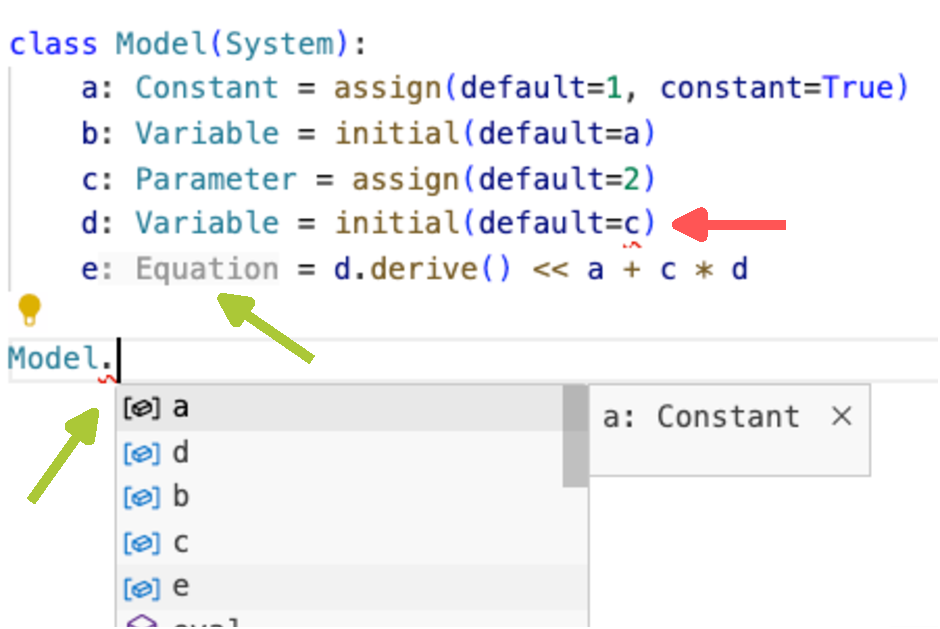
\includegraphics[width=\textwidth]{src/ide/ide1.pdf}
  }
  \end{minipage}%
  %
  \begin{minipage}[b]{0.50\linewidth}
  {
      \centering
      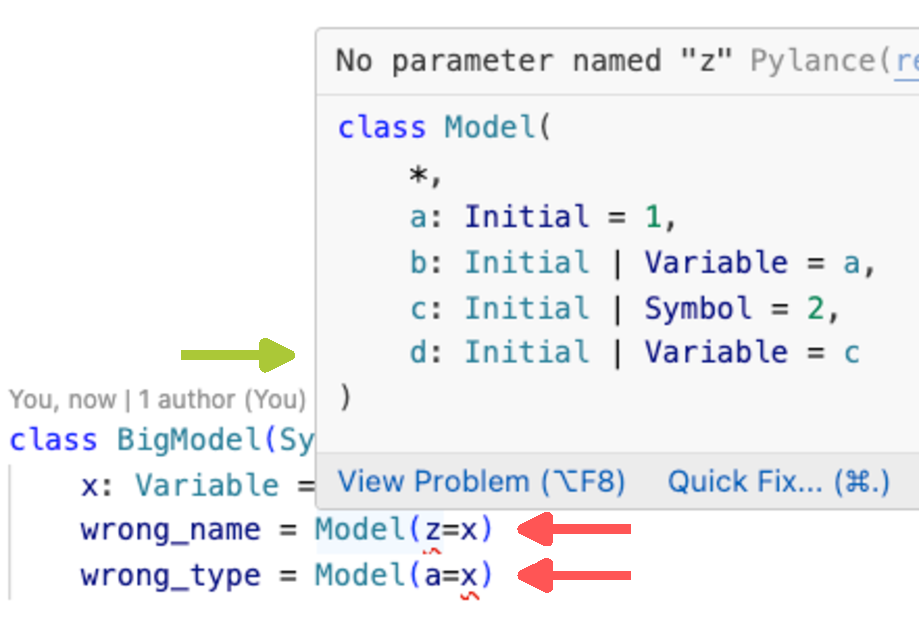
\includegraphics[width=\textwidth]{src/ide/ide2.pdf}
  }
  \end{minipage}%
  
  \caption{
      \label{fig-ide}
      Screenshots of Visual Studio Code showing
      tooltips (green arrows) and
      highlighted type errors (red arrows).
      On the left,
      we show that \texttt{a},
      a \texttt{Constant} assigned with \texttt{assign(...,\ constant=True)},
      can be used for \texttt{Variable b}'s initial condition.
      Instead,
      it is flagged as a type error (red underlining)
      when using \texttt{c}, a \texttt{Parameter},
      for \texttt{Variable d}'s initial condition,
      The IDE automatically recognizes \texttt{e} as an \texttt{Equation},
      and provides autocompletion of the \texttt{Model}'s components.
      A tooltip is shown when composing models (green arrow, right),
      which show the expected variables and their default values.
      The IDE highlights wrong names (\texttt{z} is not a name in \texttt{Model})
      and mismatched types (\texttt{x} is \texttt{Variable} and \texttt{a} must be a number or a \texttt{Constant})
  }
  
  \end{figure*}  

% FIGURE 3
\begin{figure*}[t]

  \begin{minipage}[t]{\linewidth}
  
  {\centering 
  
  \begin{CodeInput}
  \begin{Highlighting}[]
  \KeywordTok{import} \ClassTok{numpy} \KeywordTok{as} \ClassTok{np}
  \KeywordTok{from} \ClassTok{poincare} \KeywordTok{import} \ClassTok{Simulator}
  
  \VariableTok{sim} \OperatorTok{=} \ClassTok{Simulator}\KeywordTok{(\ClassTok{Oscillator})}
  \VariableTok{df} \OperatorTok{=} \VariableTok{sim}.\FunctionTok{solve}\KeywordTok{(}\VariableTok{save\_at}\OperatorTok{=}\ClassTok{np}.\FunctionTok{linspace}\KeywordTok{(}\ValueTok{0}, \ValueTok{5}, \ValueTok{101}\KeywordTok{))}
  \end{Highlighting}
  \end{CodeInput}
  
  }
  
  \end{minipage}%
  \newline
  \begin{minipage}[t]{0.45\linewidth}
  
  {\centering 
  
  \begin{CodeInput}
  \begin{Highlighting}[]
  \VariableTok{df}.\FunctionTok{head}\KeywordTok{()}
  \end{Highlighting}
  \end{CodeInput}
  
  \begin{CodeOutput}
      \begin{tabular}[]{@{}lll@{}}
          \toprule
          & x & v \\
          time & & \\
          \midrule
          0.00 & 1.000000 & 0.000000 \\
          0.05 & 0.998750 & -0.049979 \\
          0.10 & 0.995005 & -0.099835 \\
          0.15 & 0.988772 & -0.149440 \\
          0.20 & 0.980069 & -0.198672 \\
          \botrule
      \end{tabular}
  \end{CodeOutput}
      
  }
  
  \end{minipage}%
  \hfill
  \begin{minipage}[t]{0.45\linewidth}
  
  {\centering 
  
  \begin{CodeInput}
  \begin{Highlighting}[]
  \VariableTok{df}.\FunctionTok{plot}\KeywordTok{()}\OperatorTok{;}
  \end{Highlighting}
  \end{CodeInput}
  
  \begin{CodeOutput}
    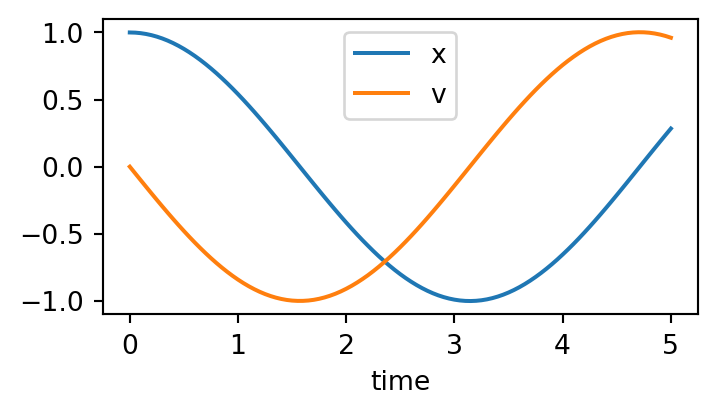
\includegraphics[width=\textwidth]{article_files/cell-9-output-1}
  \end{CodeOutput}
  
  }
  
  \end{minipage}%
  
  \caption{\label{fig-sim}Simulation of the \texttt{Oscillator} system
  from Figure~\ref{fig-second-order}. The output is a
  \texttt{pandas.DataFrame} with a column for each variable and the time
  as index. It is inspected and plotted with the \texttt{pandas} methods.}
  
  \end{figure*}
  


% FIGURE 4
\begin{figure*}[t]

  \begin{minipage}[t]{\linewidth}
    \centering 
    \begin{CodeInput}
    \begin{Highlighting}[]
    \KeywordTok{from}\ClassTok{ simbio }\KeywordTok{import}\ClassTok{ Compartment, MassAction, Species, RateLaw, \FunctionTok{initial}}
    \end{Highlighting}
    \end{CodeInput}
  \end{minipage}%
  \newline
  \begin{minipage}[t]{\linewidth}
    \centering 
    \begin{minipage}[c]{0.60\linewidth}
      \centering 
      \begin{CodeInput}
      \begin{Highlighting}[]
        \KeywordTok{class}\ClassTok{ Model}\KeywordTok{(}\ClassTok{Compartment}\KeywordTok{)}:
            \CommentTok{"""2A {-}\textgreater{} B"""}
        
        \VariableTok{    A}: \ClassTok{Species }\OperatorTok{=}\FunctionTok{ initial}\KeywordTok{(}\VariableTok{default}\OperatorTok{=}\ValueTok{1}\KeywordTok{)}
        \VariableTok{    B}: \ClassTok{Species }\OperatorTok{=}\FunctionTok{ initial}\KeywordTok{(}\VariableTok{default}\OperatorTok{=}\ValueTok{0}\KeywordTok{)}
        \VariableTok{    r }\OperatorTok{=}\ClassTok{ RateLaw}\KeywordTok{(}
        \VariableTok{        reactants}\OperatorTok{=}\KeywordTok{[}\ValueTok{2} \OperatorTok{*}\VariableTok{ A}\KeywordTok{]},
        \VariableTok{        products}\OperatorTok{=}\NormalTok{\KeywordTok{[}B\KeywordTok{]},}
        \VariableTok{        rate}\OperatorTok{=}\ValueTok{1}\NormalTok{,}
        \KeywordTok{    )}
      \end{Highlighting}
      \end{CodeInput}
    \end{minipage}%
    %
    \begin{minipage}[c]{0.40\linewidth}
      \centering 
      \[
      \begin{cases}
          \frac{dA}{dt} = -2 \\
          \frac{dB}{dt} = +1
      \end{cases}
      \begin{cases}
          A(0) &= 1 \\
          B(0) &= 0
      \end{cases}
      \]
    \end{minipage}%
  \end{minipage}%
  \newline
  \begin{minipage}[t]{\linewidth}
      \centering 
      \begin{minipage}[c]{0.60\linewidth}
          \centering 
          \begin{CodeInput}
          \begin{Highlighting}[]
          \KeywordTok{class}\ClassTok{ Model}\KeywordTok{(}\ClassTok{Compartment}\KeywordTok{)}:
              \CommentTok{"""2A {-}\textgreater{} B"""}
          
          \VariableTok{    A}: \ClassTok{Species }\OperatorTok{=}\FunctionTok{ initial}\KeywordTok{(}\VariableTok{default}\OperatorTok{=}\ValueTok{1}\KeywordTok{)}
          \VariableTok{    B}: \ClassTok{Species }\OperatorTok{=}\FunctionTok{ initial}\KeywordTok{(}\VariableTok{default}\OperatorTok{=}\ValueTok{0}\KeywordTok{)}
          \VariableTok{    r }\OperatorTok{=}\ClassTok{ MassAction}\KeywordTok{(}
          \VariableTok{        reactants}\OperatorTok{=}\KeywordTok{[}\ValueTok{2} \OperatorTok{*}\VariableTok{ A}\KeywordTok{]},
          \VariableTok{        products}\OperatorTok{=}\NormalTok{\KeywordTok{[}B\KeywordTok{]},}
          \VariableTok{        rate}\OperatorTok{=}\ValueTok{1}\NormalTok{,}
          \KeywordTok{    )}
          \end{Highlighting}
          \end{CodeInput}
      \end{minipage}%
      %
      \begin{minipage}[c]{0.40\linewidth}
          \centering 
          \[
          \begin{cases}
              \frac{dA}{dt} = -2 A^2 \\
              \frac{dB}{dt} = +1 A^2
          \end{cases}
          \begin{cases}
              A(0) &= 1 \\
              B(0) &= 0
          \end{cases}
          \]
      \end{minipage}%
  \end{minipage}%
  
  \caption{
    A reaction system for species \(A\) and \(B\)
    with initial conditions \(1\) and \(0\), respectively. A single reaction
    transforming \(2A\) into \(B\) is saved in variable \texttt{r}. The rate
    \(1\) is specified directly for \texttt{RateLaw}, and is proportional to
    the reactants for \texttt{MassAction}.
  }
  \label{fig-simbio}
\end{figure*}


% FIGURE 5
\begin{figure*}[t]
  \centering
  
  \begin{CodeInput}
  \begin{Highlighting}[]
  \KeywordTok{from}\ClassTok{ simbio.io }\KeywordTok{import}\ClassTok{ biomodels, sbml}

  \VariableTok{model }\OperatorTok{=}\ClassTok{ sbml}.\FunctionTok{load}\KeywordTok{(}\StringTok{"repressilator.sbml"}\KeywordTok{)}  \CommentTok{\# from existing SBML file}
  \VariableTok{model }\OperatorTok{=}\ClassTok{ biomodels}.\FunctionTok{load}\KeywordTok{(}\StringTok{"BIOMD12"}\KeywordTok{)}  \CommentTok{\# from BioModels}
  \VariableTok{model}
  \end{Highlighting}
  \end{CodeInput}
    
  \begin{CodeOutput}
      \begin{tabular}{@{}lll@{}}
          \multicolumn{3}{l}{Elowitz2000 - Repressilator} \\
          \toprule
          type & total & names \\
          \midrule
          variables  &  6 & PX, PY, PZ, X, Y, Z \\
          parameters & 17 & cell, beta, alpha0, alpha, eff, n, KM, tau\_mRNA, tau\_prot, ... \\
          equations  & 12 & Reaction1, Reaction2, Reaction3, Reaction4, Reaction5, ... \\
          \botrule
      \end{tabular}
  \end{CodeOutput}
  
  \caption{Creation of a model from a local SBML file or one uploaded to BioModels.}
  \label{fig-simbio-io}
\end{figure*}
  
% FIGURE 6
\begin{figure*}[t]
  \centering
  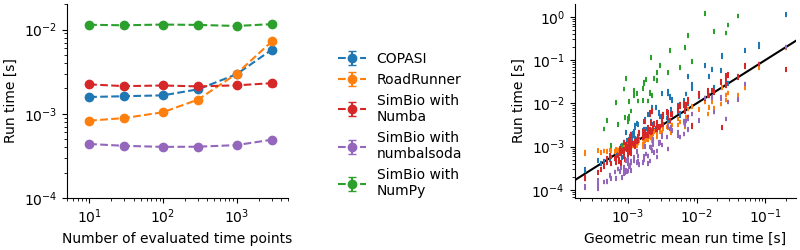
\includegraphics[width=\textwidth]{src/performance/figures/performance}
  \caption{
    Performance of different softwares to solve models from the curated section of BioModels.
    (left) Run time for the model BIOMD3 as a function of the number of output points.
    (right) Run time for different models for 300 output points,
    using the geometric mean of the different softwares to order them.
    Each point corresponds to the median of 20 runs,
    with a neglibible errorbar given by the interquartile range.
  }
  \label{fig-runtime}
\end{figure*}

\end{document}
